\documentclass[11pt, a4paper]{article}
\usepackage[top=3cm, bottom=4cm, left=3.5cm, right=3.5cm]{geometry}
\usepackage{amsmath,amsthm,amsfonts,amssymb,amscd, fancyhdr, color, comment, graphicx, environ}
\usepackage{float}
\usepackage{mathrsfs}
\usepackage{lastpage}
\usepackage[dvipsnames]{xcolor}
\usepackage[framemethod=TikZ]{mdframed}
\usepackage{enumerate}
\usepackage[shortlabels]{enumitem}
\usepackage{fancyhdr}
\usepackage{indentfirst}
\usepackage{listings}
\usepackage{sectsty}
\usepackage{thmtools}
\usepackage{shadethm}
\usepackage{hyperref}
\usepackage{setspace}
\usepackage[portuguese]{babel}
\selectlanguage{portuguese}
\hypersetup{
    colorlinks=true,
    linkcolor=blue,
    filecolor=magenta,      
    urlcolor=blue,
}
%%%%%%%%%%%%%%%%%%%%%%%%%%%%%%%%%%%%%%%%%%%%%%%%%%%%%%%%%%%%%%%%%%
%%%%%%%%%%%%%%%%%%%%%%%%%%%%%%%%%%%%%%%%%%%%%%%%%%%%%%%%%%%%%%%%%%

\mdtheorem[style=theoremstyle]{Problem}{Problem}
\newenvironment{Solution}{\textbf{Solution.}}

%%%%%%%%%%%%%%%%%%%%%%%%%%%%%%%%%%%%%%%%%%%%%%%%%%%%%%%%%%%%%%
%Page setup
\pagestyle{fancy}
\headheight 35pt
\rhead{
\includegraphics[width=2.5cm]{2_49.png}} %
\lfoot{}
\lhead{}
\pagenumbering{arabic}
\cfoot{\small\thepage}
\rfoot{}
\headsep 1.2em
\renewcommand{\baselinestretch}{1.25}       
\mdfdefinestyle{theoremstyle}{%
linecolor=black,linewidth=1pt,%
frametitlerule=true,%
frametitlebackgroundcolor=gray!20,
innertopmargin=\topskip,
}
%%%%%%%%%%%%%%%%%%%%%%%%%%%%%%%%%%%%%%%%%%%%%%%%%%%%%%%%%%%%%%%%%%
%%%%%%%%%%%%%%%%%%%%%%%%%%%%%%%%%%%%%%%%%%%%%%%%%%%%%%%%%%%%%%%%%%
%Add new commands here
\renewcommand{\labelenumi}{\alph{enumi})}
\newcommand{\Z}{\mathbb Z}
\newcommand{\R}{\mathbb R}
\newcommand{\Q}{\mathbb Q}
\newcommand{\NN}{\mathbb N}
\DeclareMathOperator{\Mod}{Mod} 
\renewcommand\lstlistingname{Algorithm}
\renewcommand\lstlistlistingname{Algorithms}
\def\lstlistingautorefname{Alg.}
%%%%%%%%%%%%%%%%%%%%%%%%%%%%%%%%%%%%%%%%%%%%%%%%%%%%%%%%%%%%%%%%%%


\begin{document}

\begin{titlepage}
    \begin{center}
        \vspace*{3cm}
            
        \Huge
        \textbf{MAP2212}
            
        \vspace{1cm}
        \huge
        Laboratório de Computação e Simulação \\
            
        \vspace{1.5cm}
        \Large
            
        \textbf{Enzo Valentim Cappelozza}     \\
        \textbf{Lucas Donaire}% <-- author
        
            
        \vfill
        
        Professor:  \\
        Julio Michael Stern
            
        \vspace{1cm}
            
        
\includegraphics[width=0.4\textwidth]{2_49.png}
        \\
        
        \Large
        
        \today
            
    \end{center}
\end{titlepage}

%%%%%%%%%%%%%%%%%%%%%%%%%%%%%%%%%%%%%%%%%%%%%%%%%%

\newpage
\section{Introdução}
Criando um programa em python com objetivo de testar hipóteses sobre um modelo bayesiano, focando nas medidas de significância \textit{e-valor} e \textit{e-valor padronizado}. Para tal, faremos uso do \textit{software Python} e das bibliotecas \textit{Scipy, Matplotlib \text{e} Math}.

\section{Testes de hipótese e nível de significância}

\subsection{p-valor}
Na vida cotidiana, são comuns as situações onde queremos estimar alguma quantia ou parâmetro desconhecido. Para tal, podemos contar com a ajuda de métodos estatísticos, que tem embasamento para inferir sobre tais objetos desconhecidos. Como nunca é possível ter certezas absolutas no que refere-se a eventos com aleatoriedade envolvida, é útil criar medidas para avaliar nossa confiança em alguma hipótese, isso é, quantificar nossa certeza que algo pode estar certo. No caso da estatística frequentista, temos o \textit{p-valor}, que mede, grosso modo, a desconfiança que temos na hipótese dadas as observações. Assim, fixamos um valor, por exemplo 5\%, e se o p-valor for menor que esse valor, mantemos a confiança na nossa hipótese (não rejeitamos a hipótese).
\subsection{e-valor}
A abordagem da estatística bayesiana se funda em outra concepção sobre como conhecemos objetos e o que podemos inferir sobre eles (outra epistemologia), então urge a necessidade de se criar uma medida bayesiana que cumpra o papel do \textit{p-valor}. Para tais funções, temos o \textbf{\textit{e-valor}}, e o \textbf{\textit{e-valor padronizado}}, que carregam propriedades interessantes e surgem a partir de uma abordagem totalmente bayesiana.

\section{Modelos Bayesianos e o e-valor}
Em um modelo Bayesiano, dada uma função a priori $r(\theta)$, calculamos a distribuição a posteriori $f(\theta | X) \propto \sum_{i=1}^{n}L(\theta|x^{(i)})p_0(x^{(i)}) $, com L a função de verossimilhança dado a amostra de tamanho i. Assim, f depende da amostra observada. Dado isso, temos as seguintes funções usadas no calculo do e-valor, função surpesa $s(\theta)$, e função verdade $W(v)$, definidas por: \\

\begin{gather*}
s(\theta) = \frac{p_n(\theta)}{r(\theta)} \\
W(v) = \int_{T(v)} p_n(\theta) d\theta, \  \text{com } \ T(v) = \{ \theta \in \Theta : s(\theta) \leq v \} \\
\end{gather*}


\subsection{Nosso modelo}
Temos um modelo trinomial de Dirichlet, onde temos as seguintes restrições no espaço amostral:
$\Theta =  \{ \theta \in \mathbb{R}^3 : (0 \leq \theta_i \leq 1, \ i = 1,2,3 ) \wedge \theta_1+\theta_2+\theta_3 =1 \} $. Assim $t = dim(\Theta) = 2$
Além disso, estamos trabalhando com a hipótese  nula
$$\Theta_0 = \{ \theta \in \Theta : \theta_3 =(1 - \sqrt{\theta_1})^2\} $$

ou seja, $ h = dim(\Theta_0) = 1$. Para testar tal hipótese, usaremos o \textit{e-valor padronizado}, $sev(\Theta_0|X)$, que será calculado utilizando a função potencial de f (em nosso código, a função \textbf{fpotential}) e a \textbf{função verdade} W(x) implementada no \textit{EP5}, junto com funções de maximização numérica, provenientes de pacotes tal como \textit{Scipy} do software \textit{Python}.  \\
A ideia, de início, é simples: como $r \propto 1$, temos que $$sup(S(\theta)) = sup(f(\theta)) = s^* = f(\theta^*)$$ 

Assim, por meio do pacote \textit{Scipy} que maximizará a nossa função potencial, podemos encontrar $\theta^*$, de maneira que seja possível obter $ev(\Theta_0|X)=W(\theta^*) $ para, finalmente, obtermos um resultado numérico para $sev(\Theta_0|X)= QQ(h,t, 1-ev(H|X)) $

\section{O programa}
Nosso estimador do \textit{EP5} estava lento e sem tanta precisão, então usamos o código de MCMC disponibilizado pelos monitores, fazendo alguns ajustes: transformamos o código em uma classe, que recebe X e Y, e constrói um objeto que tem a função U(v), que estima a função verdade W(v). Além disso, ajustamos algumas funções para evitar problemas numéricos, como por exemplo as funções que davam erro quando tentávamos calcular a função gamma em 0. Ajustamos isso alterando de 0 para 0.000001. Com essa classe, temos o que precisamos para calcular a função verdade, W(v). Assim, seguimos os seguintes passos para o calculo de sev(H|X): 


\begin{enumerate}[i)]

    \item Usa-se o \textit{Scipy} para achar $\theta^*$, ao minimizar a função potencial.
    
    \item Calcula-se $ev(\Theta_0|X) =W(s(\theta^*))$.
    
    \item Com auxilio dos módulos \textit{Scipy} e \textit{math}, pelas funcões \textit{integrate.quad} e \textit{gamma}, programa-se as funções \textit{QQ}, \textit{Chi2} e \textit{Gamma}, tais como descritas no vídeo do EP6.
    
    \item Calcula-se $sev(\Theta_0|X) = 1-QQ(t,h,1-ev)$ por meio do passo anterior, com $t=2, \ h=1$.
    
    \item Define e utiliza-se um critério para a tomada de decisão.
    
\end{enumerate}

 
\subsection{Critérios para tomada de decisão}

Definiremos o critério de aceitação/rejeição de nossa hipótese, isto é, aceitar ou rejeitar a nossa hipótese nula de acordo com a seguinte definição: 

\begin{center}
"Se $sev(\Theta_0|X) \geq 0.05$, aceitamos $\Theta_0$. Caso contrário, rejeitamos $\Theta_0$."
\end{center}


Essa escolha foi feita pois sabemos que se nossa hipótese for verdadeira, temos  $sev(\Theta_0|X) \rightarrow U_{[0,1]}$, assim, a probabilidade do erro de tipo 1 é de 0,05. Caso a hipótese seja falsa, $sev(\Theta_0|X) \rightarrow 0$, o que implica que a probabilidade do erro tipo 2 também é baixa.
 
 
 
\subsection{Maximizando/minimizando a função}
Fora feito o uso do método \textit{optimize.minimize\_scalar} para maximizar a nossa "função potencial alterada"\ definida em nosso conjunto de Hipótese Nula:

$$\Theta_0 = \{ \theta \in \Theta : \theta_3 = (1-\sqrt{\theta_1})^2  \}$$

Tornando, assim, a nossa função potencial , originalmente um campo escalar com $n=3$, uma função escalar com $n=1$ cujos valores $x = (x_1, x_2, x_3)$ e $y = (y_1 , y_2, y_3)$ encontram-se fixos, e é denotada por:  $f: \Theta_0 \rightarrow \mathbb{R}$

$$
f_{scalar}(\theta_1 \ | \ x,y) =  2\theta_1(\sqrt{\theta_1} - \theta_1)(1-\sqrt{\theta_1})^2
$$

Claramente, pelas condições do problema, isto é, $\theta \in S_3$, devemos limitar o domínio onde nossa otimização ocorrerá. Dado que temos as coordenadas $\theta_2, \ \theta_3$ em função de $\theta_1$, podemos limitar o domínio da otimização em função da nossa primeira entrada do vetor. Em outras palavras, a condição para limites (\textit{bounds}) pode ser facilmente descrita como o conjunto:

$$B = \{ \theta_1 \in \mathbb{R} : 0 \leq \theta_1 \leq 1 \}$$ assim, a função a ser maximizada encontra-se totalmente definida por:

$$f_{pot}: B \rightarrow \mathbb{R}, \ f_{pot} \equiv f_{scalar} $$

Note, no entanto, que a rotina a ser utilizada tem por finalidade a \textbf{minimização} de uma função escalar. No entanto, para maximizar $f_{pot}$ basta definir outra função $g$ com o mesmo domínio e contradomínio, tal que $g = -f_{pot}$ e, assim, minimizar $g$ e tomar o ponto $\theta^*$ como sendo o ponto de mínimo de $g$, respectivamente, o ponto de máximo de $f_{pot}$. 
    
Abaixo, algumas representações visuais obtidas por meio do método descrito acima, tal como os respectivos vetores $\theta^*$ e os parâmetros $x,y$ fixados.


Note abaixo: pela simetria do problema em questão (dado o nosso domínio definido) tomamos o vetor $y = (0,0,0)$ e variamos somente $x$.

\begin{figure}[H]
\centering
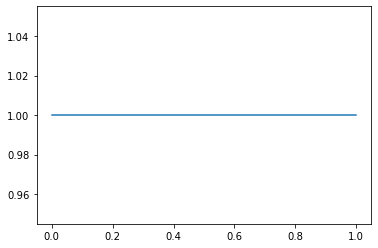
\includegraphics[scale = 0.5]{1 - 111,111.png}
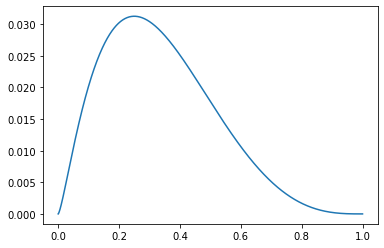
\includegraphics[scale = 0.5]{2 - 222,000.png}
\caption{Parâmetros $x = (1,1,1)$, $x=(2,2,2)$, respectivamente.}
\end{figure}

\begin{figure}[H]
\centering
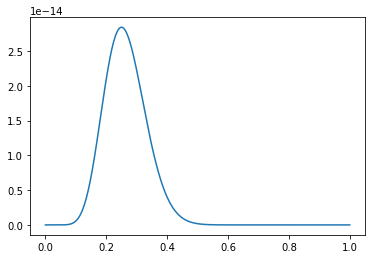
\includegraphics[scale = 0.5]{3 - 101010,000.png}
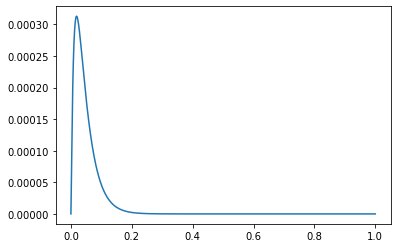
\includegraphics[scale = 0.5]{4 - 2210,000.png}
\caption{Parâmetros $x = (10, 10, 10)$, $x=(2,2,10)$, respectivamente.}
\end{figure}

\begin{figure}[H]
\centering
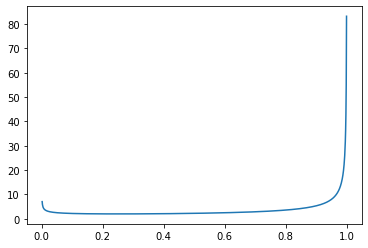
\includegraphics[scale = 0.5]{5 - 0.80.80.8, 000.png}
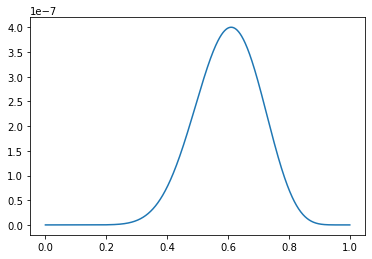
\includegraphics[scale = 0.5]{6 - 12e4e3, 000.png}
\caption{Parâmetros $x = (0.8,0.8,0.8)$, $x=(12,4,3)$, respectivamente.}
\end{figure}


E os pontos de máximo e mínimo para as imagens acima representadas são: 

\begin{center}
\begin{tabular}{|c|c|c|c|}
\hline
$x / \theta$  & $\theta_1$ & $\theta_2$ & $\theta_3$ \\
\hline
(1,1,1) & 0.9999940391390134 & 5.960852103581438e-06 &  8.882992400222503e-12 \\
\hline
(2,2,2) & 0.24999995953604695 &  0.4999999999999968 &  0.25000004046395624 \\
\hline
(10,10,10) & 0.24999991856367804 & 0.4999999999999868 & 0.2500000814363352 \\
\hline 
(2,2,10) & 0.018596216520092607 &  0.23554345766796936 & 0.7458603258119381\\
\hline 
(0.8,0.8,0.8) & 0.9999940391390134 &  5.960852103581438e-06 & 8.882992400222503e-12 \\ 
\hline 
(12, 4,3) & 0.6103514941168086 &  0.34179692423589536 &  0.04785158164729606 \\
\hline
\end{tabular}
\end{center}


\newpage
\section{Resultados e conclusão}
Sumarizamos nossos resultados na tabela a seguir, e o \textit{e-valor} computado coincidiu com os do professor Júlio. A mudança no vetor Y alterou a decisão em 6 dos 36 casos, ou 8,3\%, então pode-se dizer que Y tem sim certo nível de significância no resultado do modelo. Tivemos 36 casos onde aceitamos a hipótese, e 36 casos nos quais rejeitamos.






\begin{center}
\begin{tabular}{|c|c|c|c|c|c|c|}
\hline
x1 & x3 & Y & s(θ*) & ev(H|X) & sev(H|X) & H \\
\hline
1 & 2 & 1 & 0.1980 & 0.0033 & 0.1104 & True \\
1 & 2 & 0 & 0.0235 & 0.0004 & 0.1108 & True \\
1 & 3 & 1 & 0.6520 & 0.0133 & 0.1091 & True \\
1 & 3 & 0 & 0.1123 & 0.0021 & 0.1106 & True \\
1 & 4 & 1 & 1.6768 & 0.0394 & 0.1054 & True \\
1 & 4 & 0 & 0.3776 & 0.0078 & 0.1098 & True \\
1 & 5 & 1 & 3.5825 & 0.0918 & 0.0979 & True \\
1 & 5 & 0 & 1.0036 & 0.0226 & 0.1078 & True \\
1 & 6 & 1 & 6.6071 & 0.1837 & 0.0841 & True \\
1 & 6 & 0 & 2.2445 & 0.0533 & 0.1034 & True \\
1 & 7 & 1 & 10.7909 & 0.3120 & 0.0638 & True \\
1 & 7 & 0 & 4.3925 & 0.1103 & 0.0952 & True \\
1 & 8 & 1 & 15.8893 & 0.4830 & 0.0361 & False \\
1 & 8 & 0 & 7.7266 & 0.1935 & 0.0826 & True \\
1 & 9 & 1 & 21.3669 & 0.6652 & 0.0109 & False \\
1 & 9 & 0 & 12.4589 & 0.2994 & 0.0658 & True \\
1 & 10 & 1 & 26.4833 & 0.8345 & 0.0004 & False \\
1 & 10 & 0 & 18.6980 & 0.4246 & 0.0455 & False \\
1 & 11 & 1 & 30.4487 & 0.9527 & 0.0000 & False \\
1 & 11 & 0 & 26.4445 & 0.5673 & 0.0234 & False \\
1 & 12 & 1 & 32.5990 & 0.9998 & 0.0000 & False \\
1 & 12 & 0 & 35.6316 & 0.6969 & 0.0077 & False \\
1 & 13 & 1 & 32.5427 & 0.9613 & 0.0000 & False \\
1 & 13 & 0 & 46.2206 & 0.8111 & 0.0009 & False \\
1 & 14 & 1 & 30.2394 & 0.8453 & 0.0002 & False \\
1 & 14 & 0 & 58.3872 & 0.8989 & 0.0000 & False \\
1 & 15 & 1 & 25.9996 & 0.6671 & 0.0107 & False \\
1 & 15 & 0 & 72.9320 & 0.9578 & 0.0000 & False \\
1 & 16 & 1 & 20.4135 & 0.4696 & 0.0383 & False \\

\end{tabular}
\end{center}

\begin{center}
    \begin{tabular}{|c|c|c|c|c|c|c|}
1 & 16 & 0 & 92.5127 & 0.9872 & -0.0000 & False \\
1 & 17 & 1 & 14.2383 & 0.2794 & 0.0691 & True \\
1 & 17 & 0 & 127.6973 & 0.9980 & -0.0000 & False \\
1 & 18 & 1 & 8.2772 & 0.1285 & 0.0925 & True \\
1 & 18 & 0 & 314.7248 & 0.9958 & -0.0000 & False \\
5 & 0 & 1 & 0.7551 & 0.0151 & 0.1088 & True \\
5 & 0 & 0 & 0.0000 & 0.0005 & 0.1108 & True \\   
5 & 1 & 1 & 3.5825 & 0.0901 & 0.0981 & True \\
5 & 1 & 0 & 1.0036 & 0.0236 & 0.1076 & True \\
5 & 2 & 1 & 8.8031 & 0.2944 & 0.0666 & True \\
5 & 2 & 0 & 4.2955 & 0.1300 & 0.0922 & True \\
5 & 3 & 1 & 14.8341 & 0.6038 & 0.0183 & False \\
5 & 3 & 0 & 9.5815 & 0.3913 & 0.0509 & True \\
5 & 4 & 1 & 19.1457 & 0.8889 & 0.0000 & False \\
5 & 4 & 0 & 14.7167 & 0.7316 & 0.0048 & False \\
5 & 5 & 1 & 20.0328 & 1.0000 & -0.0000 & False \\
5 & 5 & 0 & 17.3444 & 0.9673 & -0.0000 & False \\
5 & 6 & 1 & 17.5503 & 0.8992 & 0.0000 & False \\
5 & 6 & 0 & 16.5563 & 0.9701 & -0.0000 & False \\
5 & 7 & 1 & 13.1123 & 0.6643 & 0.0110 & False \\
5 & 7 & 0 & 13.1745 & 0.7712 & 0.0024 & False \\
5 & 8 & 1 & 8.4298 & 0.4057 & 0.0486 & False \\
5 & 8 & 0 & 8.8595 & 0.4894 & 0.0351 & False \\
5 & 9 & 1 & 4.6694 & 0.2064 & 0.0806 & True \\
5 & 9 & 0 & 5.0457 & 0.2508 & 0.0736 & True \\
5 & 10 & 1 & 2.2144 & 0.0859 & 0.0987 & True \\
5 & 10 & 0 & 2.4111 & 0.1027 & 0.0963 & True \\
9 & 0 & 1 & 9.6303 & 0.1998 & 0.0816 & True \\
9 & 0 & 0 & 0.0000 & 0.0101 & 0.1095 & True \\
9 & 1 & 1 & 21.3669 & 0.6655 & 0.0108 & False \\
9 & 1 & 0 & 12.4589 & 0.3004 & 0.0657 & True \\
9 & 2 & 1 & 24.2754 & 0.9922 & -0.0000 & False \\
9 & 2 & 0 & 21.7310 & 0.8429 & 0.0003 & False \\
9 & 3 & 1 & 18.5469 & 0.8533 & 0.0002 & False \\
9 & 3 & 0 & 19.4133 & 0.9674 & -0.0000 & False \\
9 & 4 & 1 & 10.5449 & 0.4899 & 0.0351 & False \\
9 & 4 & 0 & 11.5734 & 0.6124 & 0.0172 & False \\
9 & 5 & 1 & 4.6694 & 0.2041 & 0.0809 & True \\
9 & 5 & 0 & 5.0457 & 0.2524 & 0.0734 & True \\
9 & 6 & 1 & 1.6391 & 0.0628 & 0.1021 & True \\
9 & 6 & 0 & 1.6612 & 0.0710 & 0.1009 & True \\
9 & 7 & 1 & 0.4553 & 0.0145 & 0.1089 & True \\
9 & 7 & 0 & 0.4117 & 0.0145 & 0.1089 & True \\  
\hline
    
    
    
    \end{tabular}
    
\end{center}



%\bibliographystyle{unsrt}
%\bibliography{bibliografia}

\end{document}


